\chapter{Cascades of Transducers}
\label{chap-cassys}

This chapter presents the \textit{CasSys} tool, which provides users the possibility to create cascades of Unitex transducers and new opportunities to work on natural language whith Finite State Graphs. A \textit{cascade of transducers} \index{Cascade of transducers} applies several FSGraphs (also called automata or transducers), one after the other, onto a text: each graph modifies the text, and changes can be useful for further processings with the next graphs. Such a system is typically used for syntactic analysis, chunking, information extraction, recognizing named entities etc. To do that, CasSys uses a succession of "locate pattern" commands with special options and behaviors.

\bigskip
\noindent The first prototype of the \textit{CasSys} \index{CasSys} system was created in 2002 at the LI 
(Computer science Laboratory of Université François Rabelais Tours, France) \cite{these-nathalie}. This prototype was totally  dedicated to named entity recognition. Later, CasSys was generalized to allow any sort of work needing a cascade: throughout the years,  it was improved but never really integrated in Unitex, until a recent project which resulted in the complete integration of CasSys in Unitex\footnote{"Feder-Région Centre Entités  nommées et nommables" managed by Denis Maurel, LI, Tours, France, integration carried out by Nathalie Friburger and David Nott.}.

\bigskip
\noindent Unitex grammars are known as Context free grammars and contain the notion of transduction derived from the field 
of finite state automata. A grammar with transduction (a transducer) is enabled to produce some ouput. 
CasSys is dedicated to the application of transducers in the form of a cascade.

\bigskip
\noindent Transducers are interesting because they associate a recognized sequence to informations found in the outputs of the graphs. 
These outputs can:
\begin{itemize}
	\item	Be merged with the recognized sequence and appear in the resulting concordance or modified text. 
	\item	Replace the recognized sequence to modify the text. 
\end{itemize}
\noindent These two operations transform the text or add information inside the text. 


\bigskip
\noindent  
In this chapter, we will explain how to create/modify cascades of transducers and how to apply them. Then, we deal with options and behaviors offered by CasSys.

%%%%%%%%%%%%%%%%%%%%%%%%%%%%%%%%%%%%%%%%%%%%%%%%%%%%%%%%%%%%%
\section{Applying a cascade of transducers with CasSys}
\label{section:applyCascade}
Applying a cascade of transducers consists in the modelling of linguistic phenomena in several transducers listed in a specific order to apply on a text: CasSys and its interface into Unitex permits to do this. This section explains how to use the interface to create, manage (order, add, delete) graphs and apply the cascade.   

%%%%%%%%%%%%
\subsection{Creating the list of transducers}
\label{subsec:listTrans}

\bigskip
\noindent 
In order to manage the list of transducers, the FSGraph menu proposes two submenus: "\textit{New cascade}" and "\textit{Edit cascade...}" (Figure \ref{fig13-08}). You can choose "\textit{new cascade}" to create a new list of transducers. If you want to modify an existing cascade, you can choose "\textit{Edit cascade}" to open a file explorer and choose the cascade to be opened. 

\begin{figure}[!htb]
 \centering
 \includegraphics[width=4cm]{resources/img/fig13-08.png}
 \caption{"FSGraph" menu of Unitex and submenus "\textit{New cascade}" and "\textit{Edit cascade...}"}
 \label{fig13-08}
\end{figure}

In the language directory, there is a directory named CasSys where the cascade configuration files are stored. Those files are text files with the extension \textit{.csc} (ex: mycascade.csc).

%%%%%%%%%%%%
\subsection{Editing the list of transducers}
\label{subsec:editlistTrans}

The CasSys configuration window (Figure \ref{fig13-03}) is divided into three parts :

\begin{figure}[!htb]
  \centering
  \includegraphics[width=16cm]{resources/img/fig13-03.png}
  \caption{CasSys configuration window with a list of transducers on the right hand side}
  \label{fig13-03}
\end{figure}

\begin{enumerate}
	\item a \textit{file explorer} at the left of the frame permits to select the transducers to place in the cascade. 
	The file explorer only displays \verb+fst2+ files (all the graphs you want to place in the list of transducers must be compiled in the \verb+fst2+ format). 
	
	To edit the cascade, select the graphs in the file explorer at the left, then drag and drop them into the right frame of the window.
	\item A \textit{table} at the right displays the cascade: the ordered list of transducers and the selected options for each graph.
		This table is obviously empty for a new cascade. 
	 
	The different columns of this table (Figure \ref{fig13-09}) show the numbering of each graph and permit to choose its behavior:
	\begin{itemize}
		  \item \textbf{\#}: Rank of the graph/transducer in the cascade. The \verb+fst2+ file corresponding to a graph is numbered with this rank.
		  \item \textbf{Disabled}: checkbox to disable the current graph. \textit{Disabled} meaning "\textit{not applied in the cascade}". The disabled graphs appear not numbered, greyed out and in strikethrough.
			\item \textbf{Name}: The name of the graph (with extension \verb+fst2+). If you let the mouse over the name of the graph, a tooltip appears with the whole path ot the graph (from the \verb+Graphs+ directory). Graph names appear in red italics when the source file of the graph is not found.
		  \item \textbf{Merge}: Whether the transducer should be applied in merge mode in the sense of Unitex Locate pattern functionality.
			\item \textbf{Replace}: Whether the transducer should be applied in replace mode in the sense of Unitex Locate pattern functionality.
		  \item \textbf{Until fix point}: Whether the transducer should be applied one or several times until no change occurs anymore in the text, i.e.\ until a fixed point is reached (see Section~\ref{sub:AppWhiCon}).
	\end{itemize}

	\item \textit{Several buttons} in the middle for different needs: 
		\begin{itemize}
			\item \textit{"Up/Down/Top/Bottom"} buttons are used to modify the order of the transducers on the list (it moves the selected transducer in the list); 
			\textit{"Up"} and \textit{"Down"} to move the selected transducer one line up or down, and "\textit{Top}" and "\textit{Bottom}" to move the selection to the top or to the end of the list.
			\item  \textit{"Delete"} permits to remove a selected transducer from the list of transducers. 
			\item		\textit{"Add"} adds a transducer (previously selected in the explorer) onto the list. It replaces the drag and drop actions described above. 
			\item \textit{"View"} opens the selected graph either in the file explorer or in the list of transducers of the window. It is very useful to get a quick access to any transducer either to take a quick look at its content or to modify it.
			\item \textit{"Save"} and \textit{"Save as"} permit to save the list of transducers. By default, the lists of transducers are stored in the CasSys directory of the current language (e.g. English/CasSys).
			\item \textit{"Compile"} recompile all the graphs of the cascade. Very useful to avoid to recompile a graph after changes.
			\item \textit{"Disable all"} to disable all the graphs of the cascade. 
			\item \textit{"Enable all"} to enable all the graphs of the cascade. 
			\item \textit{"Close"} to close the current window.
		\end{itemize}
\end{enumerate}

\begin{figure}[!htb]
  \centering
  \includegraphics[width=7cm]{resources/img/fig13-09.png}
  \caption{The table/list of transducers}
  \label{fig13-09}
\end{figure}

	
%%%%%%%%%%%%%%%%%%%
\subsection{Applying a cascade}
\label{subsec:launchCascade}

To apply a cascade on a text, you can select the menu "\textit{Text / Apply CasSys cascade...}" (Figure~\ref{fig13-01}), which will open the CasSys window.
This submenu "\textit{Apply CasSys cascade...}" is active only if a text has previously been opened.

\begin{figure}[!htb]
 \centering
 \includegraphics[width=5cm]{resources/img/fig13-01.png}
 \caption{"\textit{Text}" menu of Unitex and submenu "\textit{Apply CasSys Cascade...}"}
 \label{fig13-01}
\end{figure}


The CasSys window (Figure \ref{fig13-02}) displays the content of the CasSys directory of the current language. You choose 
the cascade file to be applied on the text. Then, you click on the "Launch" button to apply the cascade. The file with the list of transducers is displayed only if it has \verb+.csc+ extension.

\begin{figure}[!htb]
  \centering
  \includegraphics[width=10cm]{resources/img/fig13-02.png}
  \caption{CasSys Window to launch a cascade of transducers}
  \label{fig13-02}
\end{figure}

All morphological-mode dictionaries added in your preferences are applied to your
graphs. Preferences may be edited from the main Unitex frame (\textit{info / Preferences / morphological-mode dictionaries}).

%\subsection{Sharing a cascade transducer list file}
%\label{subsec:shareCascade}
%
%In order to ease collaborating work within CasSys, a  simple export/import
%system for the cascades is provided. This possibility is offered in the "\textit{Text / Apply CasSys cascade...}" menu (Figure \ref{fig13-02}).

%To share a cascade list file, the following steps has to be fullfilled :
%\begin{enumerate}
%  \item \textbf{Export :} Select a cascade file and click the export button. (A
%  ready to share file is created in the \texttt{/CasSys/Share} repository)
%  \item Send the file to share to your colleague
%  \item \textbf{Import :} Select the imported file and click the import button.
%  (A ready to use file is created in the \texttt{/CasSys} repository)
%\end{enumerate}


%%%%%%%%%%%%%%%%%%%%%%%%%%%%%%%%%%%%%%%%%%%%%%%%%%%%%%%
\section{Details on the behavior of CasSys}

In this section, we present details about the operation of CasSys.

%%%%%%%%%%%%%
\subsection{Type of graphs used}
\label{graphs-for-cassys}

CasSys uses the compiled version of the graphs (the \verb+fst2+ files). CasSys can handle local grammars (section~\ref{syntactic-graphs}) such as those in Chapter \ref{chap-advanced-grammars}. 
The grammars used in the cascade must follow the constraints of the grammars used in Unitex.
They may use subgraphs, morphological filters, the morphological mode, and references to information in dictionaries.
 
\bigskip
\noindent CasSys does not support debug-mode \verb+fst2+ files (Section~\ref{section-debug-mode}). When you apply a graph in debug mode through the \verb+Text > Locate Pattern+ menu, the system compiles the graph into a special debug-mode format. To obtain a regular \verb+fst2+ file, compile the graph again, either with the \verb+FSGraph+ menu, or with a command line, or by unchecking the debug mode before applying the graph with \verb+Text > Locate Pattern+ menu.

\subsection{\textit{Repeat until fix point} behaviour}
\label{sub:AppWhiCon}

With this option, CasSys applies a transducer repeatedly on a text as long as occurrences are found. This behavior is selected for a graph of a cascade if the corresponding \textbf{Until fix point} checkbox is checked.
For instance, consider the very simple graph of Figure~\ref{fig:AB->A} which recognizes \emph{AB} and
replaces it with \emph{A}. 

\begin{figure}[!htb]
  \centering
  \includegraphics[width=7cm]{resources/img/AB_to_A.png}
  \caption{Transducer which modifies BA in A}
  \label{fig:AB->A}
\end{figure}

Consider the text \emph{B B B A A A}. Applying the graph \ref{fig:AB->A} onto this text with the option \emph{Until fix point} will produce the following result :\\

\begin{tabular}{|l|cccccc|r|}
\hline
initial text  &B&B&B&A&A&A&\\
\hline
iteration 1 & &B&B&A&A&A& 1 match\\
iteration 2 & & &B&A&A&A& 1 match\\
iteration 3 & & & &A&A&A& 1 match\\
iteration 4 & & & &A&A&A& 0 match\\
\hline
\end{tabular} \\

During the first three iterations, a match is found, so the graph is
applied again on the resulting text. At the fourth iteration, no match is
found, the graph is not applied again.

\textbf{Warning:} Be aware of the risk of livelock when applying this
option. For example, a transducer which recognizes \emph{A} and replaces it with
\emph{A} would be caught in a livelock if applied on the example text.

%%%%%%%%%%%%%%%%%%%%
\subsection{The Unitex rules used for the cascade}

In the cascade, each successive graph is applied following the Unitex rules:
\begin{itemize}
	\item \textit{Insertion to the left of the matched patterns}: in the merge mode, the ouput is inserted to the left of the recognized sequence.
	\item	\textit{Priority of the leftmost match}: during the application of a local grammar, overlapping occurrences are all indexed. 
	During the construction of a concordance, all these overlapping occurrences are presented but CasSys modifies the text with each 
	graph of the cascade : so it is necessary to choose among these occurrences the one that will be taken into account. To do that, the priority is given to the leftmost sequence.
	\item \textit{Priority of the longest match}: in CasSys, during the application of a graph, it is the longest sequence 
	that will be kept.
	\item	\textit{Search limitation to a certain number of occurrences}: in CasSys, this search is not limited. Such a limitation has no sense in the use of CasSys, we always index all occurrences in the text.
\end{itemize}

%%%%%%%%%%%%%%%%%%%%
\subsection{A special way to mark up patterns with CasSys}

The output of the transducers can be used to insert special information into texts, particularly to mark up recognized patterns: it is 
possible to use all the marks you want such as ( ), [], "", etc. or xml tags such as <xxx> </xxx>.

\bigskip
\noindent CasSys also offers\textit{ a special way to mark up patterns}, that offers some advantages and that we present here.  

\bigskip
\noindent Unitex splits texts into different sorts of tokens like the sentence delimiter \{S\}; the stop marker \{STOP\}; contiguous 
sequences of letters; curly-bracket-delimited lexical tags like \{aujourd'hui,.ADV\}, etc.
The lexical tag is used by CasSys in a special way. The lexical tag (between curly brackets) is normally used to avoid ambiguities (see Sections~\ref{tokenization} and \ref{section-displaying-sentence-automata}). 
For example, if the token \emph{\{curly brackets,.N\}} is in a text, neither "curly" nor "brackets" will be recognized but the whole sequence 
"curly brackets" or the tag <N>.

\bigskip
\noindent A lexical tag can contain complex lexical information. For example, the sequence of codes \emph{N+Pers+Hum:fs} tags a token which is a noun, a person, a human and feminine singular. In a graph, you can look for a lexical token using the lexical codes it contains: for example, you can write lexical masks such as \emph{<N>} to search a noun, \emph{<Pers+Hum>} for a human person or simply \emph{<Pers>} (lexical masks are explained in Section~\ref{section-special-symbols}).
 
\bigskip
\noindent A cascade of transducers is interesting to locate an island of certainty first. It is necessary for such a system to avoid that previously recognized patterns be ambiguous with patterns recognized by the following graphs. To do that, you can tag the patterns of your graphs surrounding them by \emph{\{} and \emph{,.tag1+tag2+tagn\}} in the outputs of the graph (where \emph{tag1, tag2, etc.} are your own tags).

\bigskip
\noindent To explain this behavior, here is a very simple example. The text on which we work is :

\emph{bac a b c cc a b b ba ab a b bca a b c abaabc}.

\bigskip
\noindent The graph grfAB (Figure~\ref{fig13-05}) recognizes the sequence \emph{a b} in the text and tags this sequence with the lexical tag \textit{\{a b,.AB\}}. The results are merged with the text adding the outputs \emph{\{ }and \emph{,.AB\}} around \textit{"a b"} sequences. 

\begin{figure}[!htb]
  \centering
  \includegraphics[width=6cm]{resources/img/fig13-05.png}
  \caption{The graph grfAB}
  \label{fig13-05}
\end{figure}

\bigskip
\noindent The resulting text is : \emph{bac \{a b,.AB\} c cc \{a b,.AB\} b ba ab \{a b,.AB\} bca \{a b,.AB\} c abaabc}.

\bigskip
\noindent Now the pattern \emph{a b} is tagged \emph{AB}. A part (a or b alone) of this pattern cannot be recognized because of the tagging of \emph{a b}. 

\bigskip
\noindent After that graph, the cascade applies another graph named tagAB (Figure~\ref{fig13-06}). It has two paths: 
\begin{itemize}
	\item the first one to recognize the lexical mask \textit{<AB>} followed by \textit{c} and tags this sequence as \textit{ABC}.
  \item the second one to recognize and tag \textit{bca} preceeded by \textit{<AB>}. Only \textit{bca} is tagged as \textit{BCA}.
\end{itemize}

\begin{figure}[!htb]
  \centering
  \includegraphics[width=9cm]{resources/img/fig13-06.png}
  \caption{The graph tagAB}
  \label{fig13-06}
\end{figure}

\bigskip
\noindent The resulting text is : \emph{bac \{\{a b,.AB\} c,.ABC\} cc \{a b,.AB\} b ba ab \{a b,.AB\} \{bca,.BCA\} \{\{a b,.AB\} c,.ABC\} abaabc}.

% \#M
% 2.0.0 6.0.0 \{\\\{a b\\,\\.AB\\\} c,.ABC\}
% 10.0.0 12.0.0 \{a b,.AB\}
% 20.0.0 24.2.0 \{a b,.AB\} \{bca,.BCA\}
% 26.0.0 30.0.0 \{\\\{a b\\,\\.AB\\\} c,.ABC\}

\bigskip
\noindent The concordance displayed by Unitex should be like Figure~\ref{fig13-07}.

Note that for programming reasons (ambiguities between characters in the curly brackets of the lexical tags), we have no option but to place backslashes $\backslash$ before all ambiguous characters for Unitex ; that is why these symbols are protected with $\backslash$ in the concordance. 

\begin{figure}[!htb]
  \centering
  \includegraphics[width=15cm]{resources/img/fig13-07.png}
  \caption{The concordance resulting from this cascade}
  \label{fig13-07}
\end{figure}


\section{Tagging generalization graphs}
\label{graph-generalization}
Sometimes, we locate elements with the aid of triggering contexts, but we can't detect them if they appear
in another context. In order to locate such occurrences, CasSys proposes to
utilise tagging generalization graphs. These graphs contain empty boxes that the program fills automatically
by extracting from the list of tokens of the text (tokens.txt) the forms previously tagged in a given way.
By applying the resulting graphs to the text, this tagging is generalized to the other occurrencs of these forms.

\subsection{Declaration}
CasSys recognises a graph as a tagging generalization graph if the column \emph{Generalization} is
checked (Figure~\ref{fig12-3}).
\begin{figure}[!htb]
  \centering
  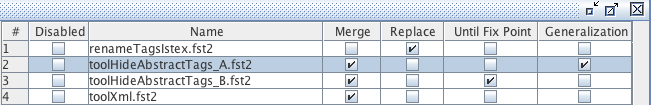
\includegraphics[width=15cm]{resources/img/fig12-3.png}
  \caption{Tagging Generalization Graph}
  \label{fig12-3}
\end{figure}

\subsection{Simple graphs}

To create a tagging generalization graph, you indicate the beginning of the generalizing part by a \$G box
with a left curly bracket in the output, and the end by an empty box with in the output a right curly bracket,
optionally preceded by features. Between these two boxes, one (and only one) empty box
must have in its output the targeted tag preceded by ",.".
You can use the \$G button (Figure~\ref{fig:bouton_g}) to automatically insert the beginning and
ending boxes of the generalizing part after selecting a box.

\begin{figure}[!htb]
  \centering
  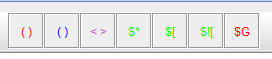
\includegraphics[width=8cm]{resources/img/bouton_g.png}
  \caption{\$G button}
  \label{fig:bouton_g}
\end{figure}

\bigskip
\noindent For example, the graph of
Figure~\ref{fig:graphe_gener_simple} is designed to generalize the \textit{x} tag.

\begin{figure}[!htb]
  \centering
  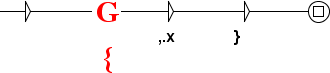
\includegraphics[width=8cm]{resources/img/graphe_generique_simple.png}
  \caption{Simple generalization graph}
  \label{fig:graphe_gener_simple}
\end{figure}

\bigskip
\noindent If the file with the token list contains the lexical tag \emph{\{A,.x\}}, the processing
will produce the graph in Figure~\ref{fig:graphe_gener_simple_genere}.

\begin{figure}[!htb]
  \centering
  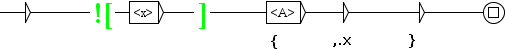
\includegraphics[width=10cm]{resources/img/graphe_generique_simple_genere.png}
  \caption{Simple generalization graph, after processing}
  \label{fig:graphe_gener_simple_genere}
\end{figure}

\bigskip
\noindent This graph will assign the \textit{x} tag to the occurrences of \emph{A} that have not received it before.
The automatically inserted negative right
context avoids tagging again already tagged occurrences. Warning:
what the program inserts into the box after the negative right context are lexical masks (see
Section~\ref{tokenization} to understand why). In case of an ambiguity between a word and a grammatical code,
they can be interpreted as grammatical codes. This is what happens with the graph
of \ref{fig:graphe_gener_simple}, which has a disastrous effect, because that of
\ref{fig:graphe_gener_simple_genere} recognizes
all the adjectives of the text!

\bigskip
\noindent Generalization graphs work only by inserting
curly-brackets-delimited lexical tags, because the forms to be tagged are extracted from the list of tokens.

\bigskip
\noindent When creating a generalization graph, several generalizing parts can be inserted in the graph, and
classic boxes can be added before and after each generalizing part, as shown in
Figure~\ref{fig:graphe_gener_plusieurs_chemins}.

\begin{figure}[!htb]
  \centering
  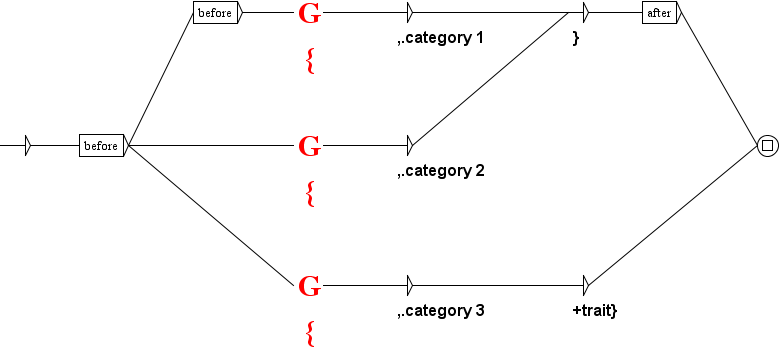
\includegraphics[width=14cm]{resources/img/graphe_generique_plusieurs_chemins.png}
  \caption{Simple generalization graph with several paths}
  \label{fig:graphe_gener_plusieurs_chemins}
\end{figure}

\subsection{Graphs with restrictions}

You may want to extract from tokens.txt the forms with a given sub-lexical tag. In the case of a token such as the following:

\bigskip
\emph{\{\{March,.month\} \{2018,.year\},.date\}}

\bigskip
\noindent we call `sub-lexical tags' the elements \emph{\{March,.month\}} and \emph{\{2018,.year\}}, and `sub-categories' the categories \textit{month} and \textit{year}.
To target the forms with a given sub-category included in forms with a given category, you can use restrictions
in generalization graphs. \footnote{ In some 3.2 alpha versions,
negative restrictions were available. They are not anymore, but the behavior of a generic part using
negative restriction can be reproduced with positive restrictions. For more information, contact the
Google Unitex list.} You type the name of the sub-category in the box, with in the output the category preceded
by ",.". \footnote{ There must be only one sub-category in the box. To extract multiple sub-categories, 
you have to create multiple generic parts.} For example, assume we want to tag more occurrences
with \textit{main} and \textit{A}, and the file tokens.txt contains the following line:

\bigskip
\emph{\{\{first,.A\} \{\{second,.A\} \{third,.B\},.B\},.main\}}

\bigskip
\begin{figure}[!htb]
  \centering
  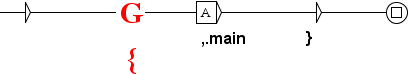
\includegraphics[width=8cm]{resources/img/graphe_restriction_A.png}
  \caption{Generalization graph with a restriction on the sub-category A}
  \label{fig:graphe_restriction_A}
\end{figure}

\bigskip
\noindent The processing of the graph in Figure~\ref{fig:graphe_restriction_A} will give the result shown in
Figure~\ref{fig:graphe_restriction_A_genere}.

\begin{figure}[!htb]
  \centering
  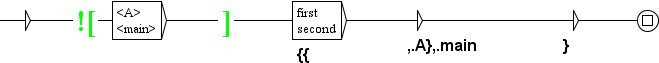
\includegraphics[width=14cm]{resources/img/graphe_restriction_A_genere.png}
  \caption{Generalization graph with a restriction on the sub-category A, after processing}
  \label{fig:graphe_restriction_A_genere}
\end{figure}

\bigskip
\noindent This graph generalizes the sub-category \textit{A} to two forms, \textit{first} and
\textit{second}. The negative right context contains the category of the main
lexical tag as well as the sub-category of the targeted sub-lexical tag. The found occurrences are
tagged twice, with both categories nested.

\begin{figure}[!htb]
  \centering
  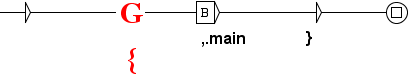
\includegraphics[width=8cm]{resources/img/graphe_restriction_B.png}
  \caption{Generalization graph with a restriction on the sub-category B}
  \label{fig:graphe_restriction_B}
\end{figure}

\bigskip
\noindent Still with the same tokens.txt file, the graph in Figure~\ref{fig:graphe_restriction_B}
will give the one in Figure~\ref{fig:graphe_restriction_B_genere}.

\begin{figure}[!htb]
  \centering
  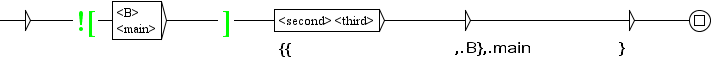
\includegraphics[width=14cm]{resources/img/graphe_restriction_B_genere.png}
  \caption{Generalization graph with a restriction on the sub-category B, after processing}
  \label{fig:graphe_restriction_B_genere}
\end{figure}

\bigskip
\noindent Only one sub-lexical tag with the sub-category \textit{B}
has been found in tokens.txt; this sub-lexical tag contains in turn two other sub-lexical tags; so the extracted content
is \textit{second third}. Because the sub-category matched,
the search was not spread to further nested sub-lexical tags, and the sub-lexical tag \textit{third} alone has not been found.

\bigskip
\noindent A generalization graph should not contain a generalizing part with a restriction and another
without restriction for the same outer category, because of the ambiguity that would result, except using weights
on the different paths (see Section~\ref{Transducers}), as shown on Figure~\ref{fig:graphe_poids}.

\begin{figure}[!htb]
  \centering
  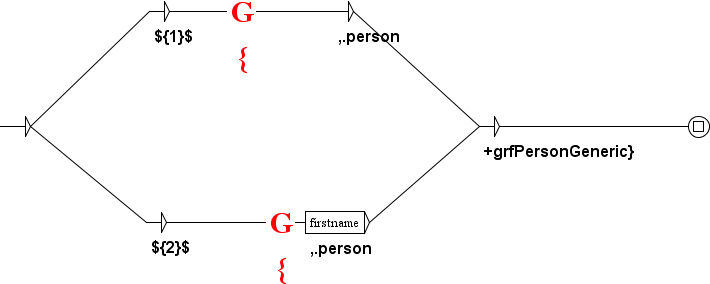
\includegraphics[width=14cm]{resources/img/graphe_poids.png}
  \caption{Graph with weights to avoid ambiguity}
  \label{fig:graphe_poids}
\end{figure}

\bigskip
\subsection{Substitution of a category}
You may want to change the outer category that will be assigned to the
sub-lexical tags extracted form the token list. For example, in the following case:

\bigskip
\noindent
\emph{\{from \{\{January,.month\} \{2017,.year\},.date\} to \{\{November,.month\} \{2018,.year\},.date\},.period\}}

\bigskip
\noindent with a generalization graph with restriction in order to extract years, the resulting sub-lexical tags would be:

\bigskip
\emph{\{\{2017,.year\},.period\}} and \emph{\{\{2018,.year\},.period\}}

\bigskip
\noindent The "period" tag is little relevant for these occurrenes. To replace it with "date",
you can indicate the final category, by appending it (separated by a dot)
to the targeted sub-category (see Figures~\ref{fig:graphe_remplacement} and
\ref{fig:graphe_remplacement_genere}).

\begin{figure}[!htb]
  \centering
  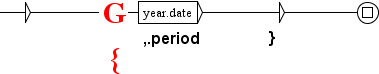
\includegraphics[width=10cm]{resources/img/graphe_remplacement.png}
  \caption{Graph with replacement of the final category}
  \label{fig:graphe_remplacement}
\end{figure}

\begin{figure}[!htb]
  \centering
  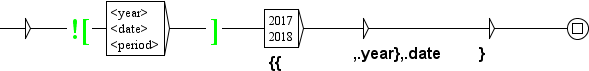
\includegraphics[width=14cm]{resources/img/graphe_remplacement_genere.png}
  \caption{Graph with replacement of the final category, after procesing}
  \label{fig:graphe_remplacement_genere}
\end{figure}

%%%%%%%%%%%%%%%%%%%%%%%%%%%%%%%%%%%%%%%%%%%%%%%%%%%%%%%%%%%%%%%%%%%
\section{The results of a cascade}

%%%%%%%%%%%%%%%%
\subsection{Displaying the concordance of a cascade}
\label{subsec:resultsCascade}

The results of a cascade are stored in an index file (\textit{concord.ind}), just as for the \textit{"Locate pattern"} operation. This index file contains all the sequences recognized using the restrictions imposed by the rules of unitex.

\bigskip
\noindent In order to display a concordance, you have to access the frame "\textit{Text / Located sequences...}" and click on the "\textit{Build concordance}" button (as described in Chapter \ref{chap-advanced-grammars}).
The figure \ref{fig13-04} presents a sample of concordance resulting of a cascade recognizing named entities. 
\begin{figure}[!htb]
  \centering
  \includegraphics[width=14cm]{resources/img/fig13-04.png}
  \caption{Concordance of CasSys under Unitex}
  \label{fig13-04}
\end{figure}

%%%%%%%%%%%%
\subsection{The different resulting files of a cascade}

CasSys keeps all the text created by each graph of the cascade. This can be useful to test, debug or check the different results of the cascade. It is possible to correct the errors on the order of the graphs or to find the errors in the writing of the graphs. A good idea is to write the name of the graph recognizing a pattern in the output of this graph: thanks to that, you can see in the final results the name of the graph by which a pattern is recognized. 
\bigskip

If you apply a cascade on the text named \texttt{example.txt}, two directories are created: \texttt{example\_snt} and \texttt{example\_csc}.
The files produced in \texttt{example\_csc} are the results obtained by each graphs. These files are named according to the number of the graph which produced them. For example, if the third graph of a cascade finds at least a pattern, the results of this graph will be stored in the directory  \texttt{example\_3\_0\_snt} and the file named \texttt{example\_3\_0.snt} will contain the modified text.

%%%%%%%%%%%
\subsection{An xml-like output text for lexical tags}

The output is provided in two forms: the direct output of the transducers, and an XML-like output with the lexical tags transformed into XML. This change is done in order to provide the end user with more easily manageable text. 
From this format, it is possible to use one of the numerous tools to process xml and it is easier to apply further transducers to get the desired output.\\
The direct output of the transducers is in the \texttt{example\_csc.raw} file. The xml-ized ouput text is copied in the \texttt{example\_csc.txt} file.

More precisely, lexical tags have the following format :\\
\begin{tabular}{c}
\texttt{
\{forme.lemme,code1+code2:flex1:flex2\}}
\end{tabular}\\
The corresponding xml-like output of CasSys has the following format :\\
\begin{tabular}{ll}
\texttt{<csc>}&\\
	&\texttt{<form>forme</form>}\\
	&\texttt{<lemma>lemme</lem>}\\
	&\texttt{<code>code1</code>}\\
	&\texttt{<code>code2</code>}\\
	&\texttt{<inflect>flex1</inflect>}\\
	&\texttt{<inflect>flex2</inflect>}\\
\texttt{</csc>}&\\
\end{tabular}

The DTD of our xml format is:

\begin{tabular}{l}
\texttt{<?xml version="1.0" encoding="ISO-8859-1"?>}\\
\texttt{<!ELEMENT text (\#PCDATA|csc)*>}\\
\texttt{<!ELEMENT csc (form,lemma?,code*,inflect*) >}\\
\texttt{<!ELEMENT form (\#PCDATA|csc)*>}\\
\texttt{<!ELEMENT lemma (\#PCDATA)>}\\
\texttt{<!ELEMENT code (\#PCDATA)>}\\
\texttt{<!ELEMENT inflect (\#PCDATA)>}\\
\end{tabular}

%%%%%%%%%%%%%%%%%%%%%%%%%%%%%%%%%%%%%%%
\section{Creating an inventory of tag occurrences}
\label{section-standOff}
The \verb$standoff$ option of CasSys (section~\ref{section-program-Cassys}) allows for processing
an XML-style tagged corpus, and producing a file that inventories the tag-delimited phrases of the 
corpus, with the number of occurrences of each unique phrase.
This option is not available via the Unitex graphical user interface. It must be launched from a script
(chapitre~\ref{chap-scripts}) or an external program.

\bigskip
\noindent You need to provide a graph that recognises the elements to be searched for (elements
in the XML sense, i.e.\ phrases delimited by an opening tag and the corresponding end tag).
Ths graph will generally involve a negative right context (section~\ref{section-contexts}). 
For example, the graph of Figure~\ref{fig-placeNameStandoff} inventories the phrases
enclosed between \verb$<placeName>$ and \verb$</placeName>$.

\begin{figure}[!htb]
  \centering
  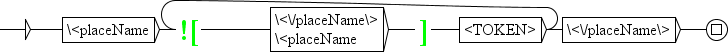
\includegraphics[width=15cm]{resources/img/placeNameStandoff.png}
  \caption{Graph for \emph{placeName}-tagged elements}
  \label{fig-placeNameStandoff}
\end{figure}

\noindent The program can process a corpus where an element contains another element with another
name,\footnote{The name of an XML element is the name in the tag.} but not a corpus where it contains another
element with the same name. 

\bigskip
\noindent To use the \verb$standoff$ option, launch a cascade containing the graph. The output is a file
with a \verb$_standoff$-suffixed name,
which lists the phrases found. It sorts them according to the element names,
and, as a secondary criterion, according to the values of the \verb$type$ attribute, if the opening tags have
it. Take for example the following tagged text:

\bigskip
\noindent \emph{<placeName type="City">Birmingham</placeName> is a populous city. \\
<placeName type="City">Birmingham</placeName> is the largest urban area of \\
<placeName type="Region">West Midlands</placeName>}.

\bigskip
\noindent By applying a cascade with the graph of Figure~\ref{fig-placeNameStandoff},
% et prenons comme option le modèle de fichier ci-dessus.
you get:
\begin{verbatim}
Tagged elements found:
     List for element "placeName" and attribute "City" 
          term="Birmingham" 
          number=2 
     End of list for this pair.
     List for element "placeName" and attribute "Region" 
          term="West Midlands" 
          number=1 
     End of list for this pair.
End of list for this corpus
\end{verbatim}

\noindent In the graph that recognises the elements, you can also restrict the values of the
\verb$type$ attribute. For example, the graph of Figure~\ref{fig-placeNameHorsRegionStandoff}
inventories the \verb$placeName$-tagged elements, except those of the \verb$Region$ type.

\begin{figure}[!htb]
  \centering
  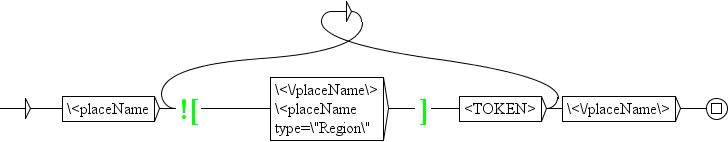
\includegraphics[width=15cm]{resources/img/placeNameHorsRegionStandoff.png}
  \caption{Graph for \emph{placeName}-tagged elements, except those of the \emph{Region} type}
  \label{fig-placeNameHorsRegionStandoff}
\end{figure}

\noindent By applying a cascade with the graph of Figure~\ref{fig-placeNameHorsRegionStandoff},
you get a result about a single pair:
\begin{verbatim}
Tagged elements found:
     List for element "placeName" and attribute "City" 
          term="Birmingham" 
          number=2 
     End of list for this pair.
End of list for this corpus
\end{verbatim}

\noindent The output file is produced on the model of a template file. Provide the name of the template file in
command line with the following syntax:

\verb$--standoff=<template file name>$

\noindent The template file is a text file with at most 10 sections:

\begin{enumerate}
\item free introductive text
\item a line with just \verb$#LINE$: the part from \verb$#LINE$ to \verb$#REST$ will be used as a template
to generate the part on an element (or on an element-type pair) in the output file
\item text introducing an element name, noted \verb${TYPE}$, and optionally a value of the
\verb$type$ attribute, noted \verb${SUBTYPE}$. The optional part must be enclosed in double angles:
\verb$<<...>>$
\item a \verb$#BLOCK$ line: the part from \verb$#BLOCK$ to \verb$#END$ will be a template for
the part on a tagged phrase in the output file
\item text introducing a tagged phrase, noted \verb${TERM}$
\item text introducing the number of occurrences of this phrase, noted \verb${COUNT}$
\item an \verb$#END$ line
\item text signalling the end of the part on an element (or on an element-type pair)
\item a \verb$#REST$ line
\item free conclusive text
\end{enumerate}

\noindent Here is the template file for the example above:
\begin{verbatim}
Tagged elements found:
#LINE
     List for element "{TYPE}"<< and attribute "{SUBTYPE}">>
#BLOCK
          term="{TERM}"
          number={COUNT}
#END
     End of list for this pair.
#REST
End of list for this corpus
\end{verbatim}

